\subsection{The topology defined by a valuation}

Let K be a not necessarily commutative field, v a valuation on K and G the totally ordered group \(v(\mathbf{K}^{*})\) . For all \(\alpha \in G\) let \(V_{\alpha}\) be the set of \(x \in K\) such that \(v(x) > \alpha\) ; this set is an additive subgroup of K ( \(\S 3\) , no. 1). There exists a unique topology \(T_{v}\) on K for which the \(V_{\alpha}\) form a fundamental system of neighbourhoods of 0 (General Topology, Chapter III, \(\S 1\) , no. 2, Example). For v to be improper, it is necessary and sufficient that \(T_{v}\) be the discrete topology.

LEMMA 1. Let \(x \in \mathbf{K}^*\) , \(y \in \mathbf{K}^*\) and \(\alpha \in \mathbf{G}\) . If

\[
v (x - y) > \sup (\alpha + 2 v (y), v (y)),
\]

then \(v(x^{-1} - y^{-1}) > \alpha\) .

\(x^{-1} - y^{-1} = x^{-1}(y - x)y^{-1}\) and hence

\[
v (x ^ {- 1} - y ^ {- 1}) = v (x - y) - v (x) - v (y).
\]

If \(v(x - y) > v(y)\) , Proposition 1 of §3, no. 1 implies that \(v(x) = v(y)\) , since \(x = y + (x - y)\) . Moreover, if \(v(x - y) > \alpha + 2v(y)\) , then

\[
v (x ^ {- 1} - y ^ {- 1}) > \alpha + 2 v (y) - 2 v (y) = \alpha .
\]

PROPOSITION 1. The topology \(\mathcal{T}_{v}\) is Hausdorff and compatible with the field structure on K. The mapping \(v: \mathbf{K}^{*} \to \mathbf{G}\) is continuous if G is given the discrete topology.

Let \(x \in \mathbf{K}^*\) and \(\alpha = v(x)\) ; then \(x \notin \mathrm{V}_{\alpha}\) , which shows that \(\mathcal{T}_v\) is Hausdorff. For all \(x_0 \in \mathbf{K}\) and \(\alpha \in \mathbf{G}\) , there exists \(\beta \in \mathbf{G}\) such that \(x_0\mathrm{V}_{\beta} \subset \mathrm{V}_{\alpha}\) and \(\mathrm{V}_{\beta}x_0 \subset \mathrm{V}_{\alpha}\) (it is sufficient to take \(\beta \geqslant \alpha - v(x_0)\) ). On the other hand, if \(\alpha \geqslant 0\) , then \(\mathrm{V}_{\alpha}\mathrm{V}_{\alpha} \subset \mathrm{V}_{\alpha}\) . The axioms \((\mathrm{AV}_{\mathrm{I}})\) and \((\mathrm{AV}_{\mathrm{II}})\) of General Topology, Chapter III, § 6, no. 3 being thus satisfied, \(\mathcal{T}_{v}\) is compatible with the ring structure on K, Let \(x_{0} \in \mathrm{K}^{*}\) ; if \(x \in \mathrm{K}^{*}\) satisfies \(v(x - x_{0}) > \sup (\alpha + 2v(x_{0}), v(x_{0}))\) , then \(v(x^{-1} - x_{0}^{-1}) > \alpha\) (Lemma 1), which shows that \(x \mapsto x^{-1}\) is continuous and that \(\mathcal{T}_{v}\) is therefore compatible with the field structure on K. Finally, the single condition \(v(x - x_{0}) > v(x_{0})\) implies \(v(x) = v(x_{0})\) (§ 3, no. 1, Proposition 1) and hence the mapping \(v: \mathrm{K}^{*} \to \mathrm{G}\) is continuous if G is given the discrete topology.

Let \(\alpha \in G\) and \(V_{\alpha}^{\prime}\) be the set of \(x \in K\) such that \(v(x) \geqslant \alpha\) . If \(\beta < \alpha\) , then \(V_{\beta} \supset V_{\alpha}^{\prime} \supset V_{\alpha}\) . If \(v\) is not improper, it is therefore seen that the \(V_{\alpha}^{\prime}\) form a fundamental system of neighbourhoods of 0 for \(\mathcal{T}_{v}\) .

The \(V_{\alpha}\) and the \(V_{\alpha}^{\prime}\) are open additive subgroups and therefore closed in K and therefore the topological field K is totally disconnected. As every non-zero ideal of the ring of v contains a \(V_{\alpha}\) , it is open and closed in K. The quotient topology on the residue field of v is therefore discrete.

\pandocbounded{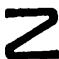
\includegraphics[keepaspectratio]{images/part003_6b42bd98.jpg}}

Let A be the ring of v. If v is discrete, Proposition 8 of §3, no. 6 shows that the topology induced by \(T_{v}\) on A is the m(A)-adic topology. This is not so in general (Exercise 4).

PROPOSITION 2. Let K be a not necessarily commutative field, v a non-improper valuation on K, A the ring of v and m the ideal of v. For K with the topology \(\mathcal{T}_v\) to be locally compact, it is necessary and sufficient that the following conditions be fulfilled:

\begin{enumerate}
\def\labelenumi{(\roman{enumi})}
\item
  K is complete;
\item
  v is discrete;
\item
  the residue field \(\kappa(A)\) is finite.
\end{enumerate}

If so, A is compact.

Suppose K is locally compact. Then it is complete (General Topology, Chapter III, § 3, no. 3, Corollary 1 to Proposition 4); further there exists a compact neighbourhood of 0, which contains a neighbourhood \(\mathbf{V}_{\alpha}^{\prime}\) , where \(\alpha\) belongs to the value group of \(v\) ; in other words, there exists \(a \neq 0\) in \(\mathbf{K}^*\) such that A.a is compact and it follows that \(\mathrm{A} = (\mathrm{A}.a)a^{-1}\) is compact. As every ideal \(\mathfrak{b} \neq (0)\) of A is open, A/b is compact and discrete (General Topology, Chapter III, § 2, no. 5, Proposition 14) and therefore finite and in particular \(\kappa(\mathrm{A}) = \mathrm{A}/\mathfrak{m}\) is finite. Moreover, for \(y \neq 0\) in \(\mathfrak{m}\) , the ring A/Ay being finite, there is only a finite number of ideals of A containing Ay and the set P of elements of the form \(v(x)\) such that

\[
0 <   v (x) \leqslant v (y)
\]

is finite; as \(v(\mathbf{K}^{*})\) is totally ordered, P has a least element \(\gamma\) . Then for all \(x \in A\) such that \(v(x) > 0\) , either \(v(x) > v(y) \geqslant \gamma\) , or \(v(x) \leqslant v(y)\) and then \(v(x) \geqslant \gamma\) by definition, so that \(\gamma\) is the least of the elements >0 of \(v(\mathbf{K}^{*})\) . As P is finite, there is a greatest integer \(m \geqslant 0\) such that \(m_{\gamma} \in P\) , whence \(m\gamma \leqslant v(y) < (m + 1)\gamma.\) We deduce that \(0 \leqslant v(y) - m\gamma < \gamma\) and by definition of \(\gamma\) this implies \(v(y) = m\gamma.\) Therefore \(v(\mathbf{K}^{*}) = \mathbf{Z}. \gamma\) and the valuation \(v\) is discrete.

Conversely, suppose conditions (i), (ii), (iii) hold. We may restrict our attention to the case where v is normed; let u be a uniformizer for v. Then \(\kappa(\mathbf{A}) = \mathbf{A}/\mathbf{A}u\) and hence A/Au is finite. As \(x \mapsto xu^{n}\) defines by taking quotients an isomorphism of the additive group A/Au onto \(Au^{n}/Au^{n+1}\) , \(A/Au^{j}\) is finite for all \(j \geqslant 0\) . As A is closed in K, it is complete and hence isomorphic to the inverse limit of the \(A/Au^{j}\) (General Topology, Chapter III, §7, no. 3, Proposition 2) and therefore compact. Since A is open in K, it is therefore seen that K is locally compact.

Remark. Note that it is sufficient in this proof to suppose that A is complete.

We shall see in § 9 that a field K fulfilling the conditions of Proposition 2 admits a centre which is either a finite algebraic extension of a p-adic field, or a field \(\mathbf{F}_{q}((\mathbf{T}))\) of formal power series over a finite field; moreover K is of finite rank over its centre.

